\documentclass[a4paper, 12pt]{article}
\usepackage[a4paper, margin=1.5cm]{geometry}
\usepackage[table, usenames, dvipsnames]{xcolor}
\usepackage{setspace}
\usepackage{graphicx}
\usepackage{subfig}
\usepackage{float}
\usepackage[style=acmnumeric, backend=biber, sorting=none]{biblatex}
\addbibresource{d4Refs.bib}
\DeclareNameAlias{author}{given-family}
\singlespacing
\usepackage{enumitem}
\setlist{nosep} % compact bullet points
% geometry based on the specificati
\newcolumntype{L}[1]{>{\raggedright\arraybackslash}p{#1}}

\usepackage{graphicx}
\usepackage{hyperref}
\usepackage{tabularx}
\usepackage{subcaption}
\usepackage{multicol}
\usepackage{longtable} % allow tables to span multiple pages
\usepackage{multirow}
\usepackage{pdfpages}
\usepackage{parskip}
\usepackage{graphicx}
\usepackage{minted}
\usepackage{dirtree}

\setminted{ frame=single, framesep=2mm, baselinestretch=1.2, fontsize=\small, breaklines,
autogobble, bgcolor=white, style=perldoc, }

% Improve table cell alignment and spacing
\usepackage{array} % for m{...} and >{\centering\arraybackslash}
\setlength{\tabcolsep}{6pt} % horizontal padding (default ~6pt)
\renewcommand{\arraystretch}{1.1} % slightly increase row height

% Reduce spacing
\setlength{\parskip}{3pt} % reduce space between paragraphs (default with parskip is ~\baselineskip)
\usepackage{titlesec}
\titlespacing*{\section}{0pt}{8pt}{4pt}
\titlespacing*{\subsection}{0pt}{6pt}{3pt}
\titlespacing*{\subsubsection}{0pt}{4pt}{2pt}

\begin{document}
    \pagestyle{empty}

    \begin{titlepage}
        \centering
        \vspace*{2cm}
        {\Huge \textbf{COMP2300}}\\[1cm]
        {\LARGE \textbf{SDDP Group 30}}\\[0.5cm]
        {\Large D7: Increment III}\\[1cm]
        {\large Date: \today}\\[0.2cm]
        {\large Version: 1.0}\\[1cm]
        \begin{tabular}{rl}
            \textbf{Group Members:} &                     \\
            Josh Wilcox             & jw14g24@soton.ac.uk \\
            Safiy Hussain           & sh6n24@soton.ac.uk  \\
            Taran McVay             & tm2n24@soton.ac.uk  \\
            Oliver Punter           & op2g24@soton.ac.uk  \\
        \end{tabular}
        \\[0.2cm]
        \vfill
    \end{titlepage}

    \section{Acceptance Criteria}

    As with the Sprint 2 acceptance criteria, We use a Gherkin-style structure because
    it makes each requirement explicit, testable, and unambiguous: \textbf{Given}
    defines the starting state or context, \textbf{When} defines the user action
    or system trigger, and \textbf{Then} defines the observable outcome that must
    be true for the story to pass. This is especially important for Increment 3
    because many of these stories involve hidden state, persistence, settings
    interactions, and cross-feature consistency rather than a single obvious UI screen.

    \subsection{Story D7-2 - Reminder Visibility Settings}

    As a user, I want to choose whether reminders use discreet or non-discreet wording
    so that reminder behaviour matches my privacy needs.

    \begin{longtable}
        {|L{0.12\textwidth}|L{0.24\textwidth}|L{0.24\textwidth}|L{0.32\textwidth}|}
        \hline \textbf{ID} & \textbf{Given} & \textbf{When} & \textbf{Then} \\
        \hline \endhead D7-2-01 & The user opens reminder settings & The settings
        page renders & A clear reminder visibility control is shown with at least
        a discreet and a non-discreet option, and each option is described in
        plain language \\
        \hline D7-2-02 & No reminder visibility preference has previously been
        saved & The app loads reminder settings for the first time & The system
        defaults to the most user-friendly mode, which is non-discreet wording \\
        \hline D7-2-03 & The user selects discreet reminder wording & The preference
        is saved & Future reminder generation uses non-specific wording that does
        not reveal sexual-health related event names or descriptions in the notification
        text \\
        \hline D7-2-04 & The user selects non-discreet reminder wording & The preference
        is saved & Future reminder generation includes the event-specific title or
        equivalent explicit identifying reminder text \\
        \hline D7-2-05 & A reminder visibility preference has been saved & The user
        closes and reopens the app & The previously selected reminder wording mode
        is restored without requiring the user to reconfigure it \\
        \hline D7-2-06 & The user changes reminder wording mode after future reminders
        have already been scheduled & The reminder system reinitialises or reschedules
        upcoming reminders & The newly selected wording mode is applied to future
        reminders rather than leaving them with stale text from the previous preference
        \\
        \hline D7-2-07 & The calculator disguise mode is enabled and discreet reminder
        wording is selected & A reminder fires & The reminder is presented in a way
        that does not undermine the disguise by using recognisable sexual-health
        text in the notification itself \\
        \hline D7-2-08 & A recurring event has multiple future reminder occurrences
        & Each reminder occurrence is triggered & Every occurrence respects the currently
        selected visibility mode rather than only the first reminder doing so \\
        \hline D7-2-09 & The stored reminder visibility preference is missing,
        corrupted, or invalid & The app initialises the reminder subsystem & The
        system falls back to discreet wording without crashing and without exposing
        explicit reminder text by accident \\
        \hline D7-2-10 & The user changes the reminder visibility mode several times
        before leaving settings & The final save occurs & The last selected option
        is the one persisted and used by the reminder system \\
        \hline
    \end{longtable}

    \subsection{Story D7-6 - Global Text-Size Scaling}

    As a user, I want a global text-size scaling setting with bounded size
    levels so that I can read the app comfortably without breaking its layout.

    \begin{longtable}
        {|L{0.12\textwidth}|L{0.24\textwidth}|L{0.24\textwidth}|L{0.32\textwidth}|}
        \hline \textbf{ID} & \textbf{Given} & \textbf{When} & \textbf{Then} \\
        \hline \endhead D7-6-01 & The user opens accessibility settings & The settings
        page renders & A global text-size control is visible with bounded size levels
        rather than an unbounded free-form value \\
        \hline D7-6-02 & The app is using its default text-size configuration & The
        user first opens the app or resets preferences & The text-size level is set
        to the documented default value \\
        \hline D7-6-03 & The user increases the text-size setting by one step & The
        new value is applied & Article list cards, headings, and body text visibly
        scale up without overlapping neighbouring elements \\
        \hline D7-6-04 & The user applies the largest supported text-size setting
        & They open an article view & The article remains readable and navigable,
        and key controls such as back, section navigation, and page indicators
        remain visible and operable \\
        \hline D7-6-05 & The user applies the largest supported text-size
        setting & They open calendar, event feed, and event detail views & Dates,
        labels, event cards, and action buttons scale appropriately without truncating
        or hiding essential content or controls \\
        \hline D7-6-06 & The user applies the largest supported text-size setting
        & They open the settings view itself & The settings controls remain fully
        operable, readable, and scrollable, so the user does not get trapped in
        an unusable configuration \\
        \hline D7-6-07 & The user decreases the text-size setting to the minimum
        supported value & The new value is applied & Text becomes smaller but
        remains legible and does not collapse spacing or produce clipped labels
        \\
        \hline D7-6-08 & The user changes text size and then navigates between
        articles, calendar, event detail, and settings & The views are rendered after
        navigation & The same text-size scale is applied consistently across those
        surfaces rather than only affecting the page where the change was made \\
        \hline D7-6-09 & The user saves a non-default text-size preference & The
        app is restarted & The chosen text-size level is restored automatically \\
        \hline D7-6-10 & The user has a non-default text-size preference stored &
        They activate reset or default behaviour & The text-size setting returns
        to the documented default and all major screens reflect that change \\
        \hline
    \end{longtable}

    \subsection{Story D7-11 - Blocked Tags, Filters, and Weighted Search}

    As a user, I want content preferences in settings and weighted search ranking
    based on those preferences so that search results better reflect what is relevant
    and what I do not want to see.

    \begin{longtable}
        {|L{0.12\textwidth}|L{0.24\textwidth}|L{0.24\textwidth}|L{0.32\textwidth}|}
        \hline \textbf{ID} & \textbf{Given} & \textbf{When} & \textbf{Then} \\
        \hline \endhead D7-11-01 & The user opens content-personalisation settings
        & The settings page renders & A blocked-tags or content-preferences section
        is shown with selectable tags or categories that can influence search and
        browsing \\
        \hline D7-11-02 & The user selects one or more blocked tags & The preference
        is saved & The blocked-tag selection is persisted locally and restored on
        app restart \\
        \hline D7-11-03 & The user has set identity or relevance preferences that
        match some article tags & They perform a search with multiple plausible results
        & Results that match the saved preferences are ranked above otherwise similar
        non-matching results \\
        \hline D7-11-04 & The user has selected blocked tags & They perform a search
        that would ordinarily return content carrying those tags & Content carrying
        blocked tags is excluded or suppressed according to the defined preference
        behaviour, and it is not treated as a normal high-ranking result \\
        \hline D7-11-05 & The user has no saved preferences at all & They
        perform a search & Search still works correctly and falls back to the
        base ranking behaviour rather than failing or producing an empty result
        set \\
        \hline D7-11-06 & A search result matches the user's preferred tags or
        identity weighting & The result card renders & The relevant matched tag
        or tags are highlighted using a visually distinct treatment so the user
        can understand why the result is relevant \\
        \hline D7-11-07 & A search result does not match any preferred tags &
        The result card renders & It is displayed without the special relevance
        highlight, so the highlighting remains meaningful and not purely decorative
        \\
        \hline D7-11-08 & The user removes a blocked tag or changes their preferences
        & They run the same search again & The result ordering and visibility update
        to reflect the new preference state rather than remaining stale from an earlier
        configuration \\
        \hline D7-11-09 & The stored preference state contains an unknown or outdated
        tag value & The search system initialises & The app ignores the invalid value
        safely, continues to search normally, and does not crash or hide unrelated
        content by mistake \\
        \hline D7-11-10 & The user searches using a term that matches both preferred
        and blocked-tag content & The results are generated & The ranking honours
        both rules in a deterministic way, so allowed preferred content is
        promoted and blocked content is not surfaced as a normal result \\
        \hline
    \end{longtable}

    \subsection{Story D7-12 - Parental Control Mode}

    As a parent or guardian, I want a parental control mode with passcode-protected
    restrictions so that blocked content remains inaccessible unless an
    authorised adult unlocks it.

    \begin{longtable}
        {|L{0.12\textwidth}|L{0.24\textwidth}|L{0.24\textwidth}|L{0.32\textwidth}|}
        \hline \textbf{ID} & \textbf{Given} & \textbf{When} & \textbf{Then} \\
        \hline \endhead D7-12-01 & The user opens parental-control settings & They
        enable parental control for the first time & They are required to create
        a passcode before parental control can become active \\
        \hline D7-12-02 & The user attempts to enable parental control with a blank,
        invalid, or incomplete passcode setup & They submit the setup form & Parental
        control is not enabled, and the user is clearly prompted to correct the
        passcode input \\
        \hline D7-12-03 & Parental control mode is active and blocked tags have
        been configured & The user performs a search & Articles carrying
        restricted tags are not shown in search results \\
        \hline D7-12-04 & Parental control mode is active & The user browses
        article feeds, recommendations, or other related discovery surfaces &
        Restricted content remains hidden there as well rather than leaking
        through non-search entry points \\
        \hline D7-12-05 & Parental control mode is active & The user attempts to
        access restricted content through a direct action or locked entry point
        & A controlled unlock flow is presented instead of opening the content
        immediately \\
        \hline D7-12-06 & The unlock flow is presented for restricted content &
        The user enters an incorrect passcode & Access remains denied, the restricted
        content stays hidden, and the app does not reveal the passcode or
        disable parental control \\
        \hline D7-12-07 & The unlock flow is presented for restricted content &
        The user enters the correct passcode & Access is granted through the
        defined unlock behaviour without corrupting the existing blocked-tag
        configuration \\
        \hline D7-12-08 & Parental control mode is active & The user attempts to
        disable it or edit the restrictions & The system requires the parental
        passcode before changing the protected settings \\
        \hline D7-12-09 & Parental control mode and its passcode have been
        configured & The app is restarted & The protected mode remains active, the
        restrictions still apply, and the user is not forced to reconfigure the
        system from scratch \\
        \hline D7-12-10 & Restricted content exists and parental mode is active
        & The user navigates through recommendations, filters, and related-content
        surfaces & Restricted items remain hidden consistently across all of
        those surfaces rather than appearing in one place but not another \\
        \hline
    \end{longtable}

    \subsection{Story D7-4 - Dark Mode and High-Contrast Display Options}

    As a user, I want dark mode and high-contrast display options so that I can choose
    a visual style that is clearer and more comfortable for me to use.

    \begin{longtable}
        {|L{0.12\textwidth}|L{0.24\textwidth}|L{0.24\textwidth}|L{0.32\textwidth}|}
        \hline \textbf{ID} & \textbf{Given} & \textbf{When} & \textbf{Then} \\
        \hline \endhead D7-4-01 & The user opens display-related accessibility settings
        & The settings page renders & A clear control is shown for at least standard
        mode, dark mode, and high-contrast mode, and the currently active mode
        is identifiable \\
        \hline D7-4-02 & No display preference has previously been saved & The
        app loads for the first time or after reset & The system defaults to the
        documented standard display mode \\
        \hline D7-4-03 & The user selects dark mode in settings & The preference
        is applied & The main app switches to a dark palette in which
        backgrounds, text, cards, and interactive controls remain legible and visually
        distinct \\
        \hline D7-4-04 & The user selects high-contrast mode in settings & The preference
        is applied & The main app switches to a higher-contrast presentation in which
        text, icons, dividers, and selected states are more visually separable
        than in standard mode \\
        \hline D7-4-05 & A non-standard display mode has been selected & The
        user navigates between article search, article view, calendar, event feed,
        event detail, and settings & The same chosen display mode is applied consistently
        across those screens rather than only affecting the settings page \\
        \hline D7-4-06 & The user is in article view while a non-standard display
        mode is active & They open navigation controls, read content, and use article
        UI affordances & Section navigation, page indicators, swipe cues, and
        article text remain readable and operable in that mode \\
        \hline D7-4-07 & The user is in the calendar or event views while a non-standard
        display mode is active & The views render event cards, dates, badges, and
        interactive buttons & Event information remains readable and controls remain
        visually distinguishable without disappearing into the background \\
        \hline D7-4-08 & The user switches directly from dark mode to high-contrast
        mode, or vice versa & The new mode is applied & The UI updates fully to
        the newly selected mode without leaving mixed colors, unreadable components,
        or stale styling from the previous mode \\
        \hline D7-4-09 & A display mode preference has been saved & The app is
        closed and reopened & The previously selected display mode is restored
        automatically rather than reverting to standard mode \\
        \hline D7-4-10 & The stored display-mode preference is missing, invalid,
        or corrupted & The app initialises its styling state & The system falls
        back safely to standard mode without crashing or producing an unreadable
        mixed-style UI \\
        \hline D7-4-11 & The user activates reset or default behaviour for
        display settings & The reset is applied & The display mode returns to
        standard mode and the change is reflected consistently across the major
        app screens \\
        \hline
    \end{longtable}

    We used the same testing process as in D6 to confirm these acceptance
    criteria, but due to verbosity decided not to include screenshots in this document.

    \section{Testing}

    Sprint 3 introduced a lot of state that lives across screens rather than on
    a single happy-path view: persisted settings, blocked tags that change
    search results, text-size and display mode preferences, recently-read
    entries with resume positions, and a discreet/non-discreet reminder mode.
    Our Sprint 3 testing effort therefore focuses on whether these are correctly
    loaded, defaulted, updated, and read back consistently by every feature that
    consumes it, rather than on a single UI screen.

    \subsection{Unit Testing}

    \textbf{What is it.} A unit test exercises a single class or method in
    isolation with an assertion that targets one specific observable outcome.

    \textbf{Why use it.} Unit tests give us the fastest feedback loop we have:
    when one fails it points at a single specific class, and they are cheap enough
    to run on every commit in the CI/CD pipeline.

    \textbf{Examples of Use.} The \texttt{ContentPreferencesServiceTest} writes to
    a temporary file per test and asserts that saving and reloading round-trips the
    selected blocked and preferred tags. On the calendar side, \texttt{RecurrenceRuleTest}
    and \texttt{CalendarEventTest} unit-test the \texttt{occursOn} logic for
    daily, weekly, monthly, and \texttt{UNTIL}-bounded recurrences, and \texttt{EventDetailFormatterTest}
    pins down the small formatting rules (dosage visible only on medication events,
    human-readable recurrence text) without loading the rest of the app.

    \subsubsection{Test Directory}

    \dirtree{%
    .1 sexualhealthapp. .2 article. .3 controller. .4 ArticleCardFactoryTest.java. .4 ArticleViewControllerTest.java. .3 model. .4 ArticleCollectionTest.java. .4 ArticleTest.java. .3 service. .4 ArticleBrowseRankingServiceTest.java. .4 ArticlePageRecommendationServiceTest.java. .4 ArticlePersonalizationServiceTest.java. .4 ArticleSearchIntegrationTest.java. .4 ArticleSearchServiceTest.java. .4 HybridSearchServiceTest.java. .4 RecentlyReadServiceTest.java. .4 RelevanceScorerTest.java. .4 SemanticSearchCacheTest.java. .4 SemanticSearchServiceTest.java. .4 TextPreprocessorTest.java. .2 calculator. .3 model. .4 CalculatorStateTest.java. .4 CalculatorTest.java. .4 SecretEquationTest.java. .3 service. .4 EquationMatcherTest.java. .4 SecretAuthServiceTest.java. .2 calendar. .3 controller. .4 CreateEventControllerTest.java. .4 EventDetailControllerTest.java. .4 EventFeedControllerTest.java. .3 model. .4 CalendarEventTest.java. .4 RecurrenceRuleTest.java. .3 service. .4 EventArticleRecommendationServiceTest.java. .4 EventStorageServiceTest.java. .3 util. .4 EventDetailFormatterTest.java. .2 mainapp. .3 controller. .4 MainAppControllerTest.java. .2 settings. .3 controller. .4 SettingsControllerTest.java. .3 service. .4 ContentPreferencesServiceTest.java. .4 DisguisePreferencesServiceTest.java. .4 ParentalControlsPinServiceTest.java. .2 util. .3 NotificationServiceTest.java. }

    \subsubsection{Screenshot}

    \begin{figure}[H] % 'h' means to place the figure here
        \centering % Center the image
        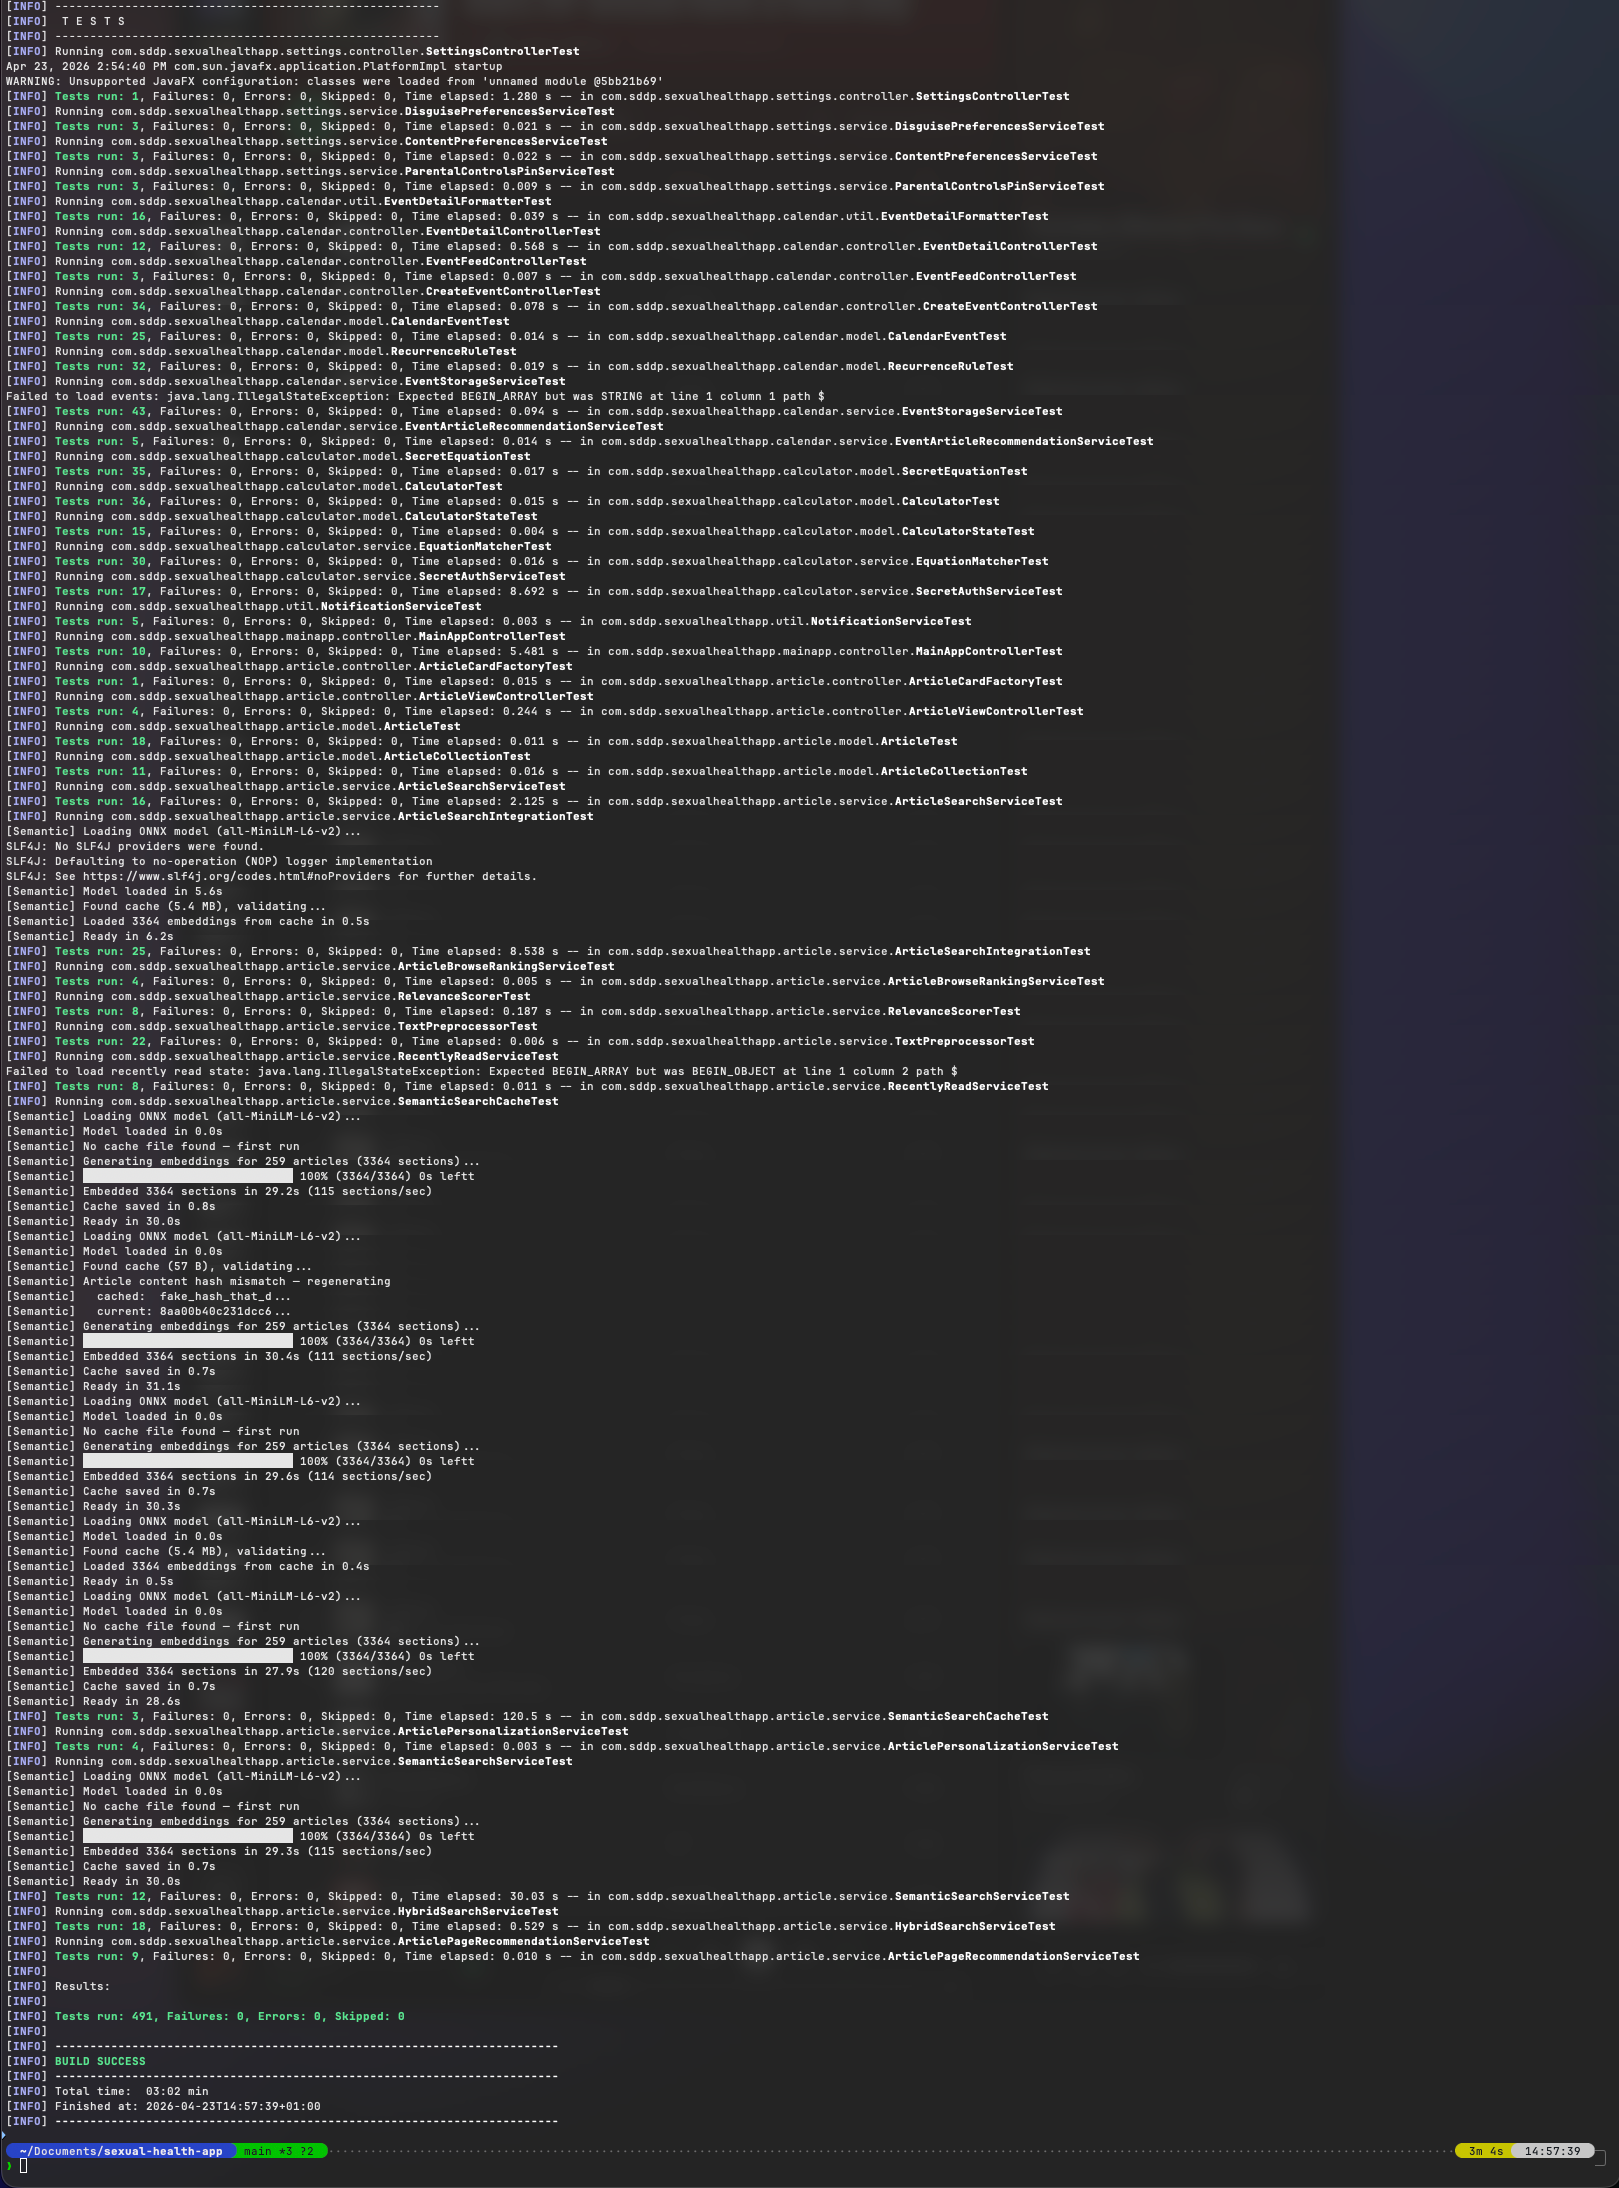
\includegraphics[width=1\textwidth]{
            figures/testscreeny.png
        } % Specify the width or height
    \end{figure}
    \subsection{Component Testing}

    \textbf{What is it.} A component test sits one level above a unit test. It
    brings together a controller with the services it directly depends on, and then
    asserts that user-visible features behave the way the acceptance criteria describe.
    It is still narrower than a full end-to-end integration test.

    \textbf{Why use it.} Our acceptance criteria are written in terms of what the
    user sees on a particular screen, and component tests are the cheapest way
    to check those at the real controller level.

    \textbf{Examples of Use.} Each component test starts JavaFX toolkit once per
    class. The test then dispatches real UI handlers (for example a card's mouse-click
    handler or a form's save action) on the JavaFx application thread and
    asserts directly on characteristics such as which view is visible or what a
    label's text reads. As an example,\texttt{EventDetailControllerTest}
    confirms that optional fields (dosage, description, recurrence) are shown or
    hidden depending on event type.

    Because these tests need a real JavaFx toolkit, they always run locally on our
    machines but are skipped on the GitLab pipeline, which does not have a
    reliable display.

    \subsection{Integration Testing}
    \textbf{What is it.} An integration test loads the real data that the live application
    uses and exercises a whole picture of the system end-to-end, across multiple
    collaborating services and through real file or scheduler state rather than
    stubs.

    \textbf{Why use it.} Every major Sprint 3 feature sits on top of a pipeline that
    spans several services. Article personalisation and ranking feed through the
    keyword, semantic, and hybrid search before they are displayed. The reminder-visibility
    setting feeds through the create-event, persist, schedule-reminder, cancel-on-delete
    features, so a wording change touches event storage and the notification scheduler
    as well as the settings service. And event-to-article suggestions pull from
    both the calendar and article features, now with the new content preferences
    layered on top. Unit tests can show that any one of those services is
    correct in isolation, but only an integration test can show that the combined
    flow (query + preferences + ranking, or event + persistence + scheduled reminder
    + cancel on edit) still produces sensible results. Integration tests stop a settings
    change from silently breaking other features.

    \textbf{Examples of Use.}

    \begin{itemize}
        \item \textbf{Articles.} \texttt{ArticleSearchIntegrationTest} loads the
            real data and checks that common queries return sensible results in correct
            score order.

        \item \textbf{Calendar and event storage.} \texttt{EventStorageServiceTest}
            persists real \texttt{CalendarEvent} objects to a temporary JSON
            file and reloads them, covering add/edit/delete, ordering, and recurrence
            expansion.

        \item \textbf{Reminder scheduling.} \texttt{NotificationServiceTest} schedules
            and cancels reminders for real events and asserts we do not get duplicates
            or ghosts.

        \item \textbf{Events meeting articles.} \texttt{EventArticleRecommendationServiceTest}
            checks that event-to-article suggestions still respect blocked/preferred
            tags .
    \end{itemize}

    \subsection{Boundary Testing}

    \textbf{What is it.} Boundary testing picks inputs that sit exactly on, just
    inside, and just outside the edge of what the system should accept. Instead of
    checking the ``nice'' middle of an input range, it picks values that are
    most likely to cause off-by-one bugs, overflow, defaults, or graceful failure.

    \textbf{Why use it.} Most regressions we caught during development were
    silent corner cases, such as ``what if the preferences file has just been deleted'',
    ``what if a reminder fires for an event that was just deleted'', ``what if a
    recurring event has an \texttt{UNTIL} date in the past'', or ``what if the user
    presses plus at the maximum text size''. Boundary tests document our
    decisions for those cases and stop them from drifting.

    \textbf{Examples of Use.}

    \begin{itemize}
        \item \textbf{Empty preferences file.} \\
            \texttt{ContentPreferencesServiceTest.missingFile\_returnsEmptyDefaults}
            asserts a missing preferences file safely defaults to \texttt{ContentPreferences.empty()}.

        \item \textbf{Corrupted JSON.} \\
            \texttt{ContentPreferencesServiceTest.invalidJson\_fallsBackToDefaults}
            asserts invalid JSON falls back safely rather than crashing.

        \item \textbf{Five-item cap on Recently Read.} \\
            \texttt{RecentlyReadServiceTest.saveProgress\_enforcesFiveItemLimit}
            asserts we keep only the 5 most recent entries and evict the oldest.

        \item \textbf{Reminder for a deleted/edited event.} \\
            \texttt{NotificationServiceTest.testDeleteEvent\_cancelsGhostNotifications}
            and \\
            \texttt{testEditEvent\_preventsDuplicateNotifications} assert
            reminders are removed on cancel and replaced on edit.

        \item \textbf{Recurring event end conditions.} \texttt{RecurrenceRuleTest}
            covers boundary cases for \texttt{UNTIL} and \texttt{COUNT} so recurrence
            expansion does not leak extra occurrences.
    \end{itemize}

    \subsection{Partitioning}

    \textbf{What is it.} Equivalence partitioning splits the input space into groups
    that the system is expected to treat the same, and then checks at least one
    representative from each group. It complements boundary testing: boundary
    picks the extreme values, partitioning picks meaningfully different categories.

    \textbf{Why use it.} A lot of Sprint 3 behaviour branches on the \textit{kind}
    of input rather than its numerical size: ``is the content preferences object
    empty, blocked-only, preferred-only, or both''; ``is this event an
    Appointment, Medication, or Test''; ``is the reminder-visibility mode discreet
    or non-discreet''; ``is the recurrence rule daily, weekly, monthly, or absent''.
    Listing every possible combination would be unreadable, so we pick one test per
    meaningful partition.

    \textbf{Examples of Use.}

    \begin{itemize}
        \item \textbf{Content preferences partitions.} \texttt{ArticlePersonalizationServiceTest}
            covers blocked-only vs preferred-only vs empty preferences.

        \item \textbf{Event type.} \texttt{EventDetailFormatterTest} and \texttt{EventDetailControllerTest}
            cover Appointment vs Medication vs Test

        \item \textbf{Recurrence pattern.} \texttt{RecurrenceRuleTest} covers none/daily/weekly/monthly
            plus \texttt{UNTIL}/\texttt{COUNT} end conditions.

        \item \textbf{Reminder visibility mode.} Discreet vs non-discreet
            wording.

        \item \textbf{Display mode.} Standard/dark/high-contrast is verified via
            manual walk-through across screens because stylesheet swaps are not
            easily unit-testable.
    \end{itemize}

    \subsection{Automated Regression Testing}

    \textbf{What is it.} The full JUnit suite is run on every push, plus locally
    before a merge request is opened.

    \textbf{Why use it.} It means that we can very easily and visually see
    breaking issues before it is merged into the main branch. And also makes accountability
    for fixing an issue very clear. \textbf{How we applied it.} We use GitLab's CI/CD
    pipeline as the backbone of our regression process. See our \texttt{.gitlab-ci.yml}
    config.

    Every merge request has to pass this pipeline before it is merged (see
    Definition of Done in the D6 report), The fix was deliberately small, and the
    same old tests stayed green afterwards, which is the regression-testing loop
    in action.

    \section{Scenario Testing}

    \subsection{How we will test using our scenarios}

    We will continue to use \textbf{scenario-based acceptance testing} to validate
    the app end-to-end from the perspective of our personas. We will still use
    the scenarios from previous deliverables, but have a couple of updated ones below
    that focus on the new features.

    \begin{itemize}
        \item \textbf{Acceptance tests}: does the scenario's goal succeed as written?

        \item \textbf{Unit tests}: the small services behind the scenario.

        \item \textbf{Regression tests}: the old tests that still need to pass after
            the Sprint 3 changes.

        \item \textbf{Boundary and partition tests}: the edge cases and category
            partitions listed in the previous section.
    \end{itemize}

    \subsection{Scenario 3.1 - Personalised search, blocked tags, and discreet
    reminders}

    People: Jamie Kendrick (29) - non-binary, queer/pansexual, nurse. Setting:
    Jamie's bedroom at home, Sunday evening. Action (goal): Jamie wants search results
    that reflect their identity, with topics they don't want to see filtered out,
    and wants reminders to stay discreet even while the calculator disguise is active.

    Jamie opens the app, enters their secret equation, and is taken to the article
    search screen. Before searching, Jamie taps the settings icon in the bottom navigation
    bar to open the new \textbf{Settings} view. On the \textbf{Content
    Preferences} card, Jamie selects a preferred tag (``LGBTQ+'') and blocks a
    tag they are not currently interested in (``Pregnancy''). The selection is saved
    immediately, and a short visual confirmation is shown.

    Jamie then switches to the \textbf{Reminder Visibility} card and selects \textbf{discreet
    wording}, because they do not want reminders for an upcoming PrEP dose to be
    identifiable on their home screen. Still inside settings, Jamie toggles on \textbf{dark
    mode} from the \textbf{Display} card, which applies immediately across
    settings itself and the rest of the app.

    Jamie returns to the main page using the back arrow and searches for ``screening
    before new partner''. The results list shows articles tagged \textbf{LGBTQ+}
    at the top with a visually distinct highlight on the matched tag. Articles tagged
    ``Pregnancy'' are not present. Jamie opens a relevant article, and returns to
    the calendar to confirm their next PrEP reminder is still on the feed. When
    the reminder fires later, its text uses the discreet wording, so neither the
    article contents nor the notification reveals what the app is about.

    \textbf{What we will test}

    \textbf{A1. Settings navigation (D7-11-01, D7-4-01, D7-2-01)}

    \begin{itemize}
        \item Given Jamie is on the main page, when the settings tab is selected,
            then the settings home renders a card for each Sprint 3 preference surface.

        \item When the Content Preferences card is tapped, the detail view
            becomes visible and the home view is hidden.
    \end{itemize}

    \textbf{A2. Persisted blocked and preferred tags (D7-11-02)}

    \begin{itemize}
        \item When Jamie selects LGBTQ+ as a preferred tag and Pregnancy as a
            blocked tag and leaves the detail view, the preferences are written to
            \texttt{content-preferences.json}.

        \item When the app is restarted, the same preferences are loaded from
            disk rather than resetting to empty.
    \end{itemize}

    \textbf{A3. Weighted ranking and blocked filtering (D7-11-03, D7-11-04)}

    \begin{itemize}
        \item Given a set of otherwise-similar articles with overlapping tags, a
            search that ordinarily returns Pregnancy-tagged content does not
            list any Pregnancy articles.

        \item Articles tagged LGBTQ+ are ranked above otherwise-similar non-matching
            articles and are rendered with a highlight on the matched tag.
    \end{itemize}

    \textbf{A4. Discreet reminder wording (D7-2-03, D7-2-07)}

    \begin{itemize}
        \item Given Jamie has selected discreet wording, when the PrEP reminder
            fires the notification uses non-specific language that does not
            mention the event title.

        \item If the calculator disguise is active, the reminder is shown in a
            way that does not undermine the disguise.
    \end{itemize}

    \textbf{A5. Dark mode consistency (D7-4-05)}

    \begin{itemize}
        \item Given dark mode is selected, when Jamie navigates between settings,
            search, article view, calendar, and event detail, each screen uses the
            dark palette and remains readable.
    \end{itemize}

    \textbf{Unit / regression tests that support scenario 3.1}

    \begin{itemize}
        \item \texttt{ContentPreferencesServiceTest}: save and reload tags,
            empty defaults, corrupted JSON fallback.

        \item \texttt{ArticlePersonalizationServiceTest}: blocked tags remove articles
            (including blocked-by-title), preferred tags boost matching results,
            highlighted tags surfaced from the query.

        \item \texttt{ArticleBrowseRankingServiceTest}: preferred tags affect ordering
            without overriding recent-read signal, no-signal fallback still
            ranks sensibly.

        \item \texttt{SettingsControllerTest}: settings home renders cards,
            tapping one opens the matching detail view.

        \item \texttt{NotificationServiceTest}: reminder scheduling/cancellation
            still behaves correctly after the D7-2 wording change.
    \end{itemize}

    \subsection{Scenario 3.2 - Accessibility-first reading and resuming}

    People: Mary Hargate (68) - retired, little confidence with technology, mild
    dyslexia. Setting: Mary's room in her care home, morning. Action (goal): Mary
    wants to continue reading an article she started yesterday, at a comfortable
    text size and in a font she can read easily, without losing her place.

    Mary opens the app, enters her secret equation, and is taken to the article search
    screen. Because she has a non-default text size and font preference saved
    from her previous session, the app loads directly into her chosen \textbf{large}
    text size with the \textbf{OpenDyslexic} font applied. At the top of the
    article feed, she sees a \textbf{Recently Read} row above \textbf{Articles
    For You}, showing the article she was reading yesterday.

    She taps her recent card, which reopens the article at the section she was last
    on (not the start). She continues reading, navigating sections using the mini
    navigation menu. When she reaches the end she returns to the feed; her progress
    on that article has updated to the latest section. She then opens the
    settings view to check the text size control, and can see that the settings controls
    themselves are still operable and scrollable at the largest supported text size,
    rather than being clipped or hidden.

    \textbf{What we will test}

    \textbf{B1. Recently Read visibility and order (D7-3)}

    \begin{itemize}
        \item Given Mary has read at least one article, when the browse feed
            renders, the Recently Read section is present and is placed above Articles
            For You.

        \item When no recent entries exist, the Recently Read section is hidden
            rather than rendered empty.

        \item When Mary performs a search, the Recently Read section is hidden
            so it does not clash with search results.
    \end{itemize}

    \textbf{B2. Resume at saved section and progress update (D7-3)}

    \begin{itemize}
        \item Given a recent card with a saved section index, when Mary taps it
            the article view opens at exactly that section.

        \item As Mary reads further sections, the saved section index updates
            without creating duplicate entries.
    \end{itemize}

    \textbf{B3. Recently Read management (D7-3)}

    \begin{itemize}
        \item When Mary uses the Clear button, the section disappears and the
            underlying JSON becomes an empty list.

        \item When she removes a single entry, only that entry disappears and
            the article itself is not opened as a side effect.
    \end{itemize}

    \textbf{B4. Text size scaling (D7-6-03, D7-6-04, D7-6-06)}

    \begin{itemize}
        \item When Mary increases the text size one step, article cards, headings,
            and body text visibly scale without overlapping.

        \item At the largest supported text size, the article view, calendar,
            event detail, and settings screens remain operable and key controls remain
            visible.
    \end{itemize}

    \textbf{B5. Font and persistence (D7-7, D7-6-09)}

    \begin{itemize}
        \item When OpenDyslexic is enabled, readable content surfaces (article body,
            card titles, settings labels) use that font consistently.

        \item When Mary closes and reopens the app, her text size and font
            choices are restored from the stored preference file.
    \end{itemize}

    \textbf{Unit / regression tests that support scenario 3.2}

    \begin{itemize}
        \item \texttt{RecentlyReadServiceTest}: new-entry creation, update
            without duplicate, newest-first ordering, five-item cap, unknown id skip,
            out-of-range section clamp, duplicate dedup, corrupted-json recovery.

        \item \texttt{MainAppControllerTest}: Recently Read hidden without entries,
            placed above Articles For You when present, hidden in search results,
            resume-at-saved-section, Clear and Remove buttons.

        \item \texttt{ArticleBrowseRankingServiceTest}: recent reads are used as
            the primary TF-IDF signal, preferred tags adjust ordering without
            overriding recent reads, fallbacks behave sanely with no signals.
    \end{itemize}

    \subsection{Scenario 3.3 Parental control and safer browsing}

    People: Alex (46) - parent of a 14-year-old (Jo from D5). Setting: the
    family living room, evening, while Jo is at school. Action (goal): Alex
    wants to configure the app on Jo's phone so that it still provides
    trustworthy sexual health information but hides tag categories they consider
    age-inappropriate, protected by a passcode that only Alex knows.

    Alex unlocks Jo's phone with her permission, opens the app via the
    calculator disguise, and navigates to the new \textbf{Settings} view. On the
    \textbf{Parental Control} card Alex chooses \textbf{enable} for the first time.
    Because no passcode has been created before, the setup flow requires Alex to
    create one before the mode activates; submitting a blank or incomplete code
    is rejected with a clear prompt.

    Once parental control is active, Alex opens the \textbf{Content Preferences}
    card and selects a set of blocked tags. They then run a test search that would
    normally return articles in one of those categories, and confirm none are
    shown. They close the app, reopen it, and confirm that parental control is still
    active and still requires the passcode to be disabled; entering an incorrect
    passcode on the unlock flow keeps the restrictions in place and does not
    reveal the passcode. Finally, Alex walks through article recommendations, related-article
    cards, and the browse feed to confirm that restricted content does not leak
    through any of those discovery surfaces.

    \textbf{What we will test}

    \textbf{C1. Passcode setup validation (D7-12-01, D7-12-02)}

    \begin{itemize}
        \item Given parental control is being enabled for the first time, when a
            valid passcode is entered, the mode activates and is persisted.

        \item When the passcode field is blank or incomplete, activation is
            blocked and a clear prompt is shown.
    \end{itemize}

    \textbf{C2. Blocked tag enforcement across surfaces (D7-12-03, D7-12-04, D7-12-10)}

    \begin{itemize}
        \item Given restricted tags are configured, a search that would normally
            return them does not list them.

        \item The same restriction is applied to the browse feed, article-to-article
            recommendations, and event-to-article recommendations, so blocked
            content does not leak through a non-search entry point.
    \end{itemize}

    \textbf{C3. Unlock flow and passcode protection (D7-12-05, D7-12-06, D7-12-07,
    D7-12-08)}

    \begin{itemize}
        \item Attempting to access restricted content opens an unlock flow rather
            than the content itself.

        \item An incorrect passcode keeps content hidden; a correct passcode
            grants access without corrupting the blocked-tag configuration.

        \item Disabling parental control or editing restrictions requires the passcode.
    \end{itemize}

    \textbf{C4. Persistence across restart (D7-12-09)}

    \begin{itemize}
        \item Given parental control and its passcode are configured, when the
            app is closed and reopened, the mode is still active and the configuration
            is not lost.
    \end{itemize}

    \textbf{Unit / regression tests that support scenario 3.3}

    The parental control feature reuses the existing content-preferences
    plumbing, so the following already-passing tests form the regression safety net:

    \begin{itemize}
        \item \texttt{ContentPreferencesServiceTest}: underlying blocked-tag storage
            and corruption handling are shared with parental control.

        \item \texttt{ArticlePersonalizationServiceTest}: blocked-tag filtering on
            search and browse surfaces.

        \item \texttt{ArticlePageRecommendationServiceTest} and \texttt{EventArticleRecommendationServiceTest}:
            confirm blocked tags also suppress article-to-article and event-to-article
            recommendations, which is what stops restricted content leaking through
            non-search entry points.
    \end{itemize}

    \section{UML Diagrams}
    \subsection{Activity Diagram}
    \begin{figure}[H]
        \centering
        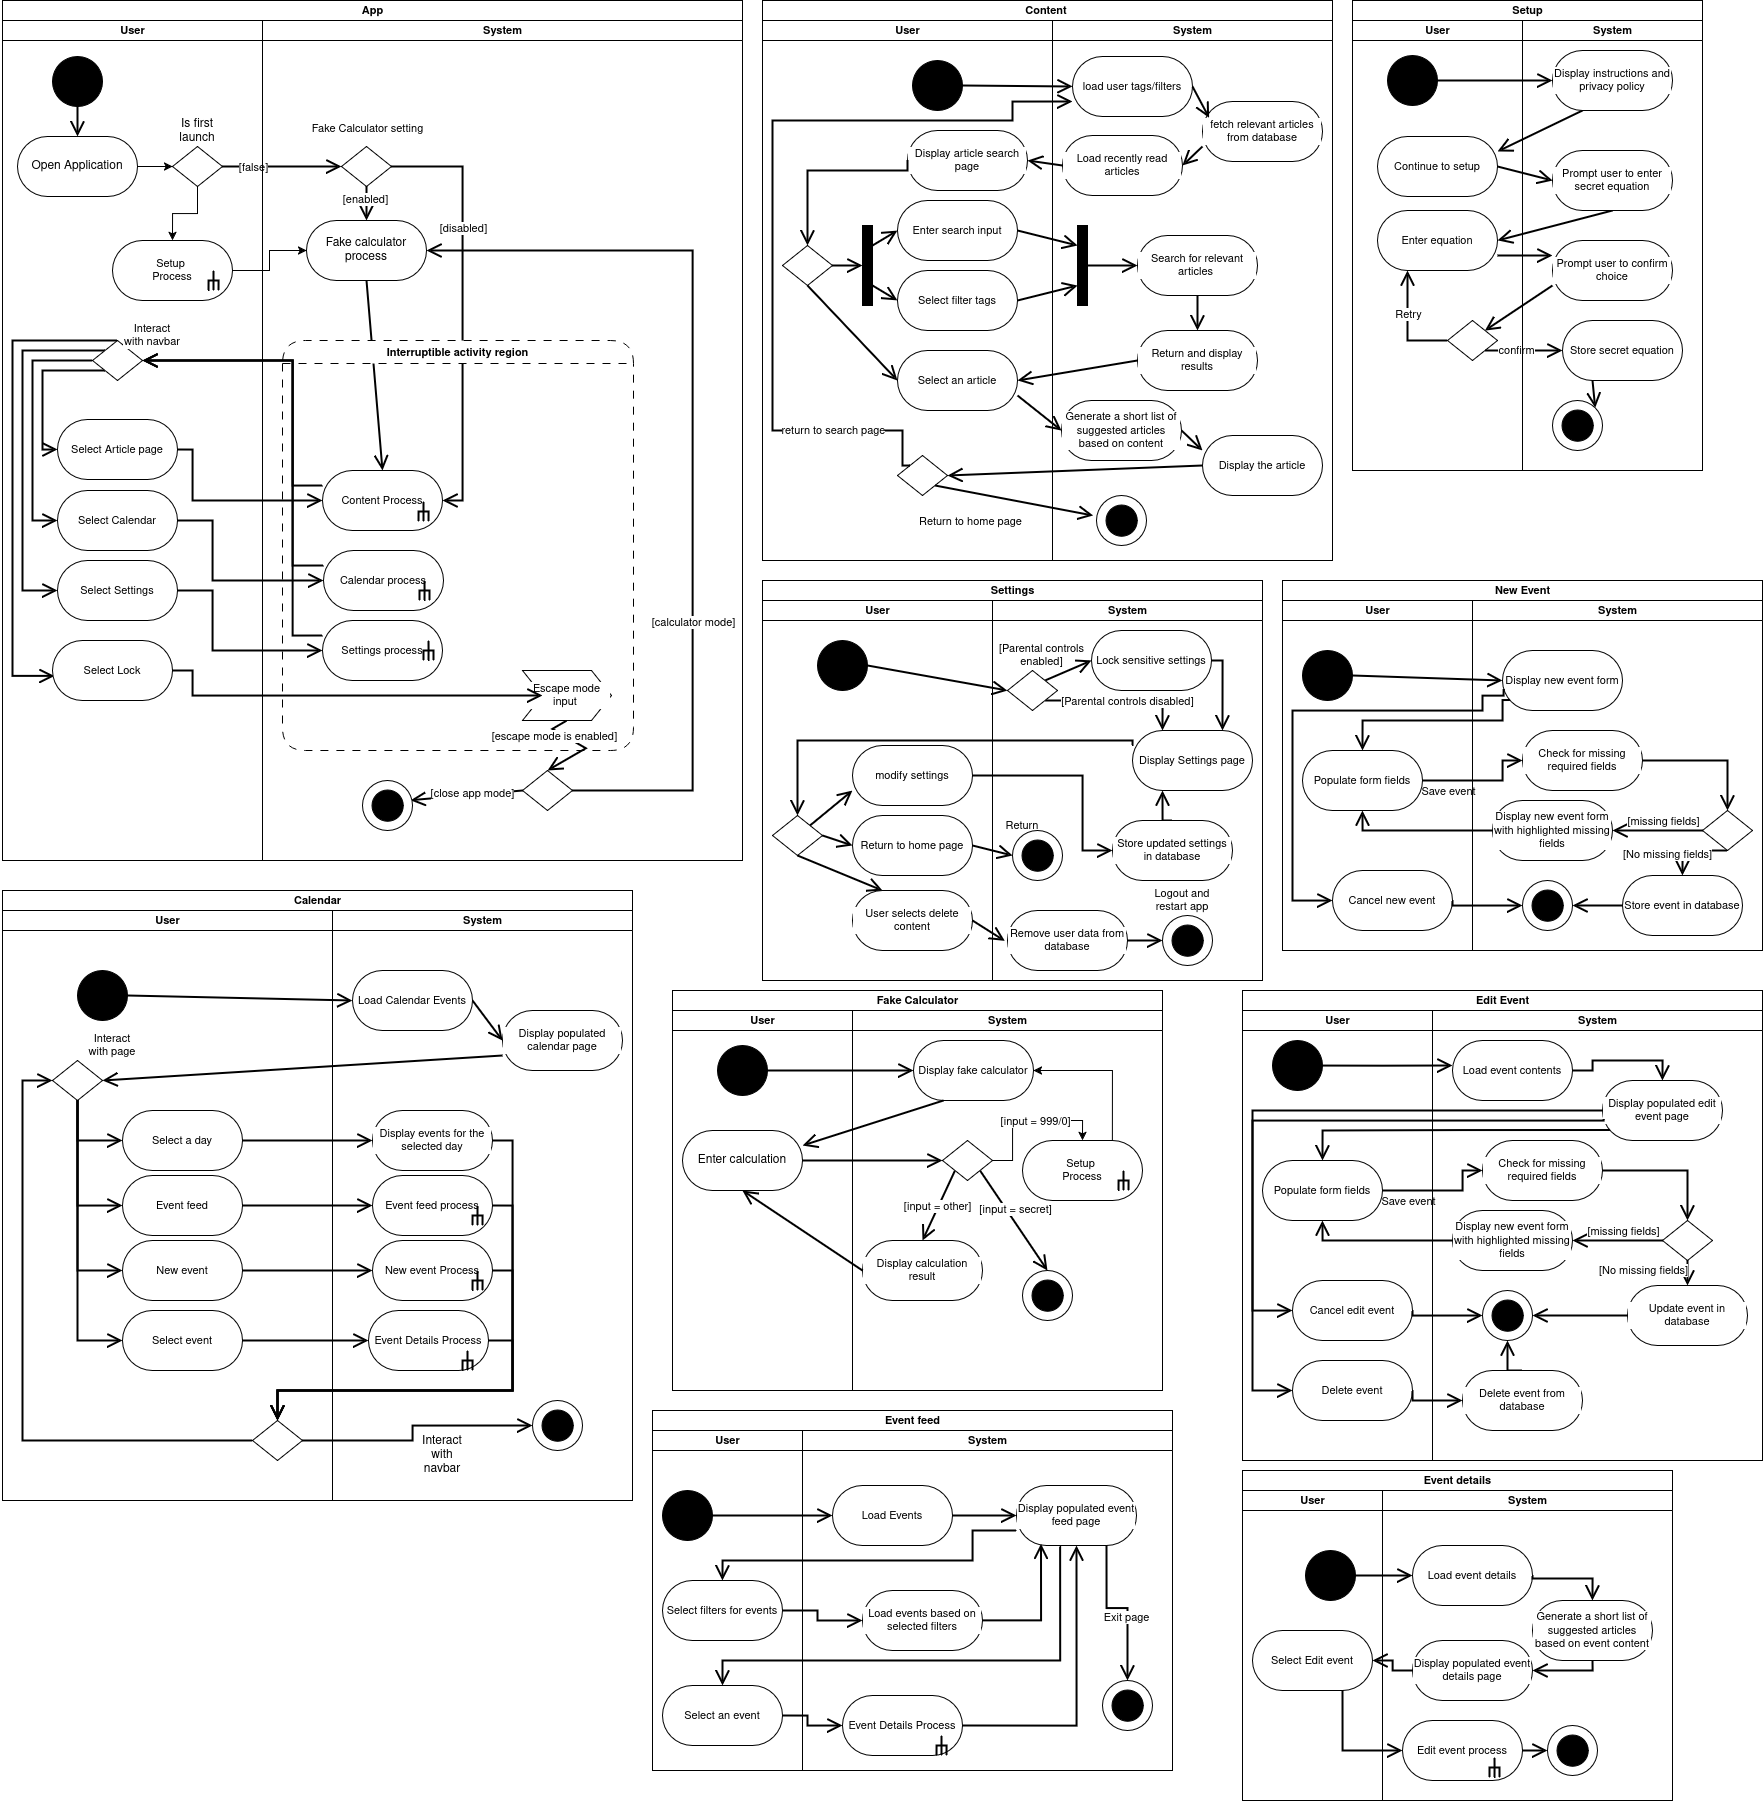
\includegraphics[width=1\linewidth]{figures/activityDiagramD7.png}
    \end{figure}

    \subsection{Class Diagram}

    \begin{figure}[H]
        \centering
        \includegraphics[width=1\linewidth]{D7//figures/d7classdiagram.png}
    \end{figure}

    \section{Sprint III review}
    \subsection{Stories}

    This sprint had a large focus on accessibility features, ensuring our app
    was able to offer value to users from many different walks of life. This included a dyslexic-friendly font, text size scaling, as well as parental controls. We also added some features to polish and round off parts of the app.

    We did not implement D7-10 from our sprint plan in D6. We realised that it would negatively impact the new user experience, by making the onboarding process a bit too lengthy and confusing. Also, its purpose would be served by our user guide as well, so it was not providing much value on its own.

    We dedicated a decent time chunk to integration, which covers all time spent on pull request and code review, as well as time spent during meetings discussing how features should be integrated together. This is tracked as D7-14 in the table below.

    \noindent
    Cell colours indicate MoSCoW prioritization: \colorbox{green!8}{Must Have} \quad
    \colorbox{blue!5}{Should Have} \quad \colorbox{yellow!5}{Could Have}

    \begin{longtable}
        {|>{\raggedright\arraybackslash}p{1cm}|>{\raggedright\arraybackslash}p{1cm}|>{\raggedright\arraybackslash}p{7.5cm}|>{\raggedright\arraybackslash}p{0.8cm}|>{\raggedright\arraybackslash}p{1.2cm}|>{\raggedright\arraybackslash}p{2cm}|>{\raggedright\arraybackslash}p{1.4cm}|}
        \hline \textbf{User Story ID} & \textbf{Task ID} & \textbf{Task
        Description} & \textbf{D} & \textbf{Story Points} & \textbf{Task Owner} &
        \textbf{Hours Spent}\\
        \hline \endfirsthead \hline \textbf{User Story ID} & \textbf{Task ID} & \textbf{Task
        Description} & \textbf{D} & \textbf{Story Points} & \textbf{Task Owner} &
        \textbf{Hours Spent}\\
        \hline \endhead

        \multirow[t]{2}{*}{D7-1} & D7-1.1 & \cellcolor{blue!5} Add a setting to enable
        or disable calculator-disguise launch mode and persist the preference locally
        & & 3 & Oli & 0.5 \\
        \cline{2-7} & D7-1.2 & \cellcolor{blue!5} Update startup routing so disabling
        disguise opens the main app directly, while preserving manual lock/disguise
        access & D7-1.1 & 2 & Oli & 0.5 \\
        \hline

        \multirow[t]{3}{*}{D7-2} & D7-2.1 & \cellcolor{yellow!8} Add reminder-visibility
        settings that let users choose discreet vs non-discreet reminder wording
        & & 3 & Oli & 1.5 \\
        \cline{2-7} & D7-2.2 & \cellcolor{yellow!8} Apply the selected reminder
        wording mode to reminder notification text generation & D7-2.1 & 3 & Oli
        & 3 \\
        \cline{2-7} & D7-2.3 & \cellcolor{yellow!8} Ensure existing reminder
        settings default safely and update correctly when users change reminder-visibility
        mode & D7-2.2 & 2 & Oli & 1.5 \\
        \hline

        \multirow[t]{4}{*}{D7-3} & D7-3.1 & \cellcolor{blue!5} Persist recently
        read article state (article ID, last read section/chunk, timestamp) & &
        4 & Josh & 0.5 \\
        \cline{2-7} & D7-3.2 & \cellcolor{blue!5} Add a "Recently Read" area in
        the article feed ordered by recency & D7-3.1 & 4 & Josh & 0.5\\
        \cline{2-7} & D7-3.3 & \cellcolor{blue!5} Reopen recently read articles at
        the saved progress position & D7-3.1 & 3 & Josh & 0.5 \\
        \hline

        \multirow[t]{3}{*}{D7-4} & D7-4.1 & \cellcolor{green!8} Add dark mode and
        high-contrast display options so users can choose a clearer visual style
        & & 3 & Safiy & 2 \\
        \cline{2-7} & D7-4.2 & \cellcolor{green!8} Add simple settings so users can
        switch between standard, dark, and high-contrast views & D7-4.1 & 3 & Safiy
        & 1 \\
        \cline{2-7} & D7-4.3 & \cellcolor{green!8} Ensure the chosen display style
        is used consistently across the main app screens & D7-4.2 & 2 & Safiy & 3.5
        \\
        \hline

        \multirow[t]{2}{*}{D7-5} & D7-5.1 & \cellcolor{yellow!8} Refactor \emph{styles.css}
        into multiple feature-oriented CSS files and update loading/import
        wiring & & 3 & Taran & 0.5 \\
        \cline{2-7} & D7-5.2 & \cellcolor{yellow!8} Remove duplicated selectors
        and verify no regressions from CSS split & D7-5.1 & 2 & Taran & 0.5 \\
        \hline

        \multirow[t]{3}{*}{D7-6} & D7-6.1 & \cellcolor{green!8} Implement a
        global text-size scaling setting with bounded size levels & & 5 & Safiy
        & 1.5 \\
        \cline{2-7} & D7-6.2 & \cellcolor{green!8} Apply increased text-size
        scaling to article, calendar/event, and settings UIs without layout
        breakage & D7-6.1 & 5 & Safiy & 4 \\
        \cline{2-7} & D7-6.3 & \cellcolor{green!8} Persist text-size preference
        and provide reset/default behavior & D7-6.1, D7-6.2 & 3 & Safiy & 1.5 \\
        \hline

        \multirow[t]{2}{*}{D7-7} & D7-7.1 & \cellcolor{blue!5} Add OpenDyslexic font
        asset and a settings toggle for enabling it & & 2 & Safiy & 0.5 \\
        \cline{2-7} & D7-7.2 & \cellcolor{blue!5} Apply OpenDyslexic font consistently
        to readable content surfaces & D7-7.1, D7-6.1 & 1 & Safiy & 1.5 \\
        \hline

        \multirow[t]{2}{*}{D7-8} & D7-8.1 & \cellcolor{blue!5} Add shape-based
        event indicators in calendar views so event types are distinguishable
        without color alone & & 2 & Taran & 0.5 \\
        \cline{2-7} & D7-8.2 & \cellcolor{blue!5} Keep indicator semantics
        consistent between calendar cells and event/feed representations & D7-8.1
        & 1 & Taran & 0.5 \\
        \hline

        \multirow[t]{2}{*}{D7-9} & D7-9.1 & \cellcolor{yellow!8} Add "suggested articles"
        cards within article views (article-to-article recommendations) & & 2 &
        Josh & 3 \\
        \cline{2-7} & D7-9.2 & \cellcolor{yellow!8} Hide the suggestion area
        when no relevant articles are available & D7-9.1 & 1 & Josh & 1 \\
        \hline

        \multirow[t]{3}{*}{D7-11} & D7-11.1 & \cellcolor{yellow!8} Add blocked
        tags / filters section in settings for user content preferences & & 3 &
        Josh & 1.5 \\
        \cline{2-7} & D7-11.2 & \cellcolor{yellow!8} Weight search ranking based
        on user tags/identity settings while respecting blocked tags & D7-11.1 &
        3 & Josh & 1.5 \\
        \cline{2-7} & D7-11.3 & \cellcolor{yellow!8} Highlight relevant matched
        tags in a distinct result color treatment & D7-11.2 & 2 & Josh & 0.5 \\
        \hline

        \multirow[t]{4}{*}{D7-12} & D7-12.1 & \cellcolor{yellow!8} Implement
        parental control mode setup with lock/passcode management & D7-11.1 & 4
        & Taran & 1 \\
        \cline{2-7} & D7-12.2 & \cellcolor{yellow!8} Enforce blocked-tag/content
        gating in search and article browsing when parental mode is active & D7-12.1,
        D7-11.2 & 4 & Taran & 0.5 \\
        \cline{2-7} & D7-12.3 & \cellcolor{yellow!8} Provide controlled unlock flow
        requiring parental passcode to access restricted content & D7-12.2 & 3 &
        Taran & 0.5 \\
        \cline{2-7} & D7-12.4 & \cellcolor{yellow!8} Ensure restricted content remains
        hidden across related recommendation/filter surfaces while parental mode
        is active & D7-12.1 & 2 & Taran & 0.5 \\
        \hline

        \multirow[t]{2}{*}{D7-13} & D7-13.1 & \cellcolor{green!8} Add privacy policy
        page in settings explaining data/storage/notification usage & & 2 & Oli &
        1 \\
        \cline{2-7} & D7-13.2 & \cellcolor{green!8} Add clear privacy policy entry
        point from onboarding/settings navigation & D7-13.1, D7-10.1 & 1 & Oli &
        0.5 \\
        \hline

        \multirow[t]{3}{*}{D7-14} & D7-14.1 & \cellcolor{green!8} Integrate the
        accessibility, personalisation, and parental-control features so
        settings from one area are respected consistently across search, article,
        and calendar flows & all & 3 & Safiy & 2 \\
        \cline{2-7} & D7-14.2 & \cellcolor{green!8} End-to-end integration
        testing across the Sprint 3 feature pipeline, verifying settings persistence,
        content filtering, reminder visibility options, and recently-read
        behaviour in one unified flow & all & 3 & Taran & 2.5 \\
        \cline{2-7} & D7-14.3 & \cellcolor{blue!5} Integrate onboarding/settings
        guidance with the new feature set and verify users can discover and
        return to key controls without breaking navigation state & all & 2 &
        Josh & 2.5 \\
        \hline
    \end{longtable}

    \subsection{Burndown Chart}
    \begin{figure}[H]
        \centering
        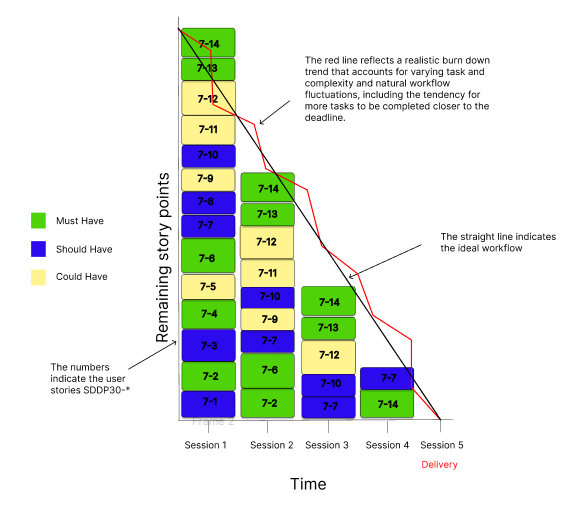
\includegraphics[width=1.0\textwidth]{
            figures/d7_completed_burndown.png
        }
        \caption{Completed Sprint 3 Burndown Chart}
    \end{figure}

    The completed burndown chart shows that the team made steady progress across
    the sprint and finished all planned Sprint 3 stories by the delivery point. The
    actual burndown line did not follow the ideal line exactly, but this is
    expected in Agile development because work is rarely completed at a
    perfectly constant rate. Instead, progress happened in stages, with larger drops
    occurring when related tasks were fully integrated and closed together.

    In the early part of the sprint, the remaining story points decreases more
    slowly than the ideal trend, suggesting the implementation work was still being
    developed in parallel and some tasks were not ready to be marked complete yet.
    This is typical when stories depend on shared components such as settings
    persistence, UI integration and cross section consistency. From Sessions 2
    to 4, the burndown dropped more sharply, showing that the team began
    completing and integrating major stories such as display settings, text size
    scaling, blocked tags and parental controls.
    \section{Group Report}
    \subsection{Summary of Work Completed}
    In Deliverable 7, we focused on making the app more personalised. The sprint
    built on the article, calendar, event, and settings features from the
    previous deliverables, but instead of adding only isolated screens, we
    introduced settings that affect behaviour across the whole app.

    The main work completed was reminder visibility settings, global text size scaling,
    blocked and preferred tags for article personalisation, parental control mode,
    and display accessibility options such as dark mode and high contrast mode. These
    features all introduced persistent state, meaning the app had to remember a
    user's preferences and apply them consistently after restart and across
    different screens.

    Overall, this deliverable moved the app forward from being mainly functional
    to being more adaptable to different user needs. It improved privacy through
    parental controls, improved accessibility through text size and display settings
    and improved relevance through personalised article filtering and ranking.
    \subsection{Report on Specific Tasks that Make up D7}
    \subsubsection{Implementation}

    First, we added reminder visibility settings so users can choose between
    discreet and non discreet reminder wording. This meant creating a settings control,
    storing the user's choice persistently, and making sure future reminders used
    the correct wording.

    Second, we implemented global text size scaling using a fixed set of size
    levels rather than a free text value. This required updating article pages,
    search results, calendar views, event screens, and settings so text could grow
    or shrink without breaking the layout or hiding controls.

    Third, we introduced content personalisation through blocked and preferred
    tags. Users can now block topics they do not want to see and prioritise tags
    that are more relevant to them. This affected article browsing, search ranking
    and recommendations and also required clear visual feedback so users could understand
    why certain results were highlighted or prioritised.

    Fourth, parental control mode was implemented with a passcode protected
    restriction system. This prevented restricted content from appearing in search,
    browse, and related content surfaces unless unlocked by an authorised user.

    Finally, we added standard, dark and high contrast display modes. These had
    to be applied consistently across article search, article view, calendar ,
    event feed , event detail and settings. A lot of refinement was needed here to
    ensure that text, cards , buttons, badges and overlays stayed readable across
    all themes.
    \subsubsection{Testing}
    We used the same overall testing strategy as in D6, but in D7 the emphasis was
    much on persistence, defaults, fallback behaviour and consistency between screens.

    \textbf{Unit tests} were used to verify smaller services such as saved
    preferences , recurrence behaviour, reminder logic, and formatting rules. \textbf{Component
    tests} checked controller behaviour and whether the right UI state appeared
    under different conditions. \textbf{Integration tests} were important
    because many of these new features depend on several services working
    together, for example saved content preferences affecting article ranking,
    or reminder visibility settings affecting future scheduled notifications.

    We also used \textbf{boundary testing} for edge cases such as missing or corrupted
    saved settings, invalid stored values, and recurrence limits. \textbf{Partition
    testing} was useful for checking meaningful categories like discreet versus non
    discreet reminders, blocked only versus preferred only content settings and
    standard versus dark versus high contrast display modes.

    Automated \textbf{regression tests} were run through \textbf{CI/CD} pipeline
    so we could catch failures whenever new settings related features were added.

    \subsubsection{User Guide}
    We created instructions covering first launch, secret equation setup,
    article browsing, calendar and event management, settings and reminder/privacy
    features. This was important because this sprint introduced a larger number of
    persistent settings and cross screen behaviour, so the app could no longer
    rely on users discovering everything through trial and error alone.

    Creating the guide also helped us validate the usability of the system
    itself. Writing step by step instructions exposed places where feature behaviour
    needed to be explained more clearly, particularly around blocked tags ,
    parental controls, reminder visibility and accessibility options such as display
    mode and text size scaling. In that sense, the user guide was not just documentation
    produced at the end, but also lightweight usability check on whether the
    application's flows were understandable from a user perspective.
    \subsection{Planning and Management}
    We continued to use an \textbf{Agile Scrum} style workflow for this
    deliverable. Work was organised into Sprint 3 user stories, each with
    explicit acceptance criteria written in a \textbf{Gherkin style} format.
    This was especially useful in D7 because many user stories involved hidden
    state, saved settings, and behaviour that spans several parts of the app
    rather than one obvious UI screen.

    We also shifted our task coordination from Jira to Git-based project
    organisation during this deliverable. Instead of relying primarily on a separate
    planning board, we used branches, commit history, merge requests to organise
    work and track progress more directly alongside the codebase

    We also used \textbf{burndown} tracking to monitor progress across the
    sprint. As in the previous sprint, implementation of individual tasks was
    manageable, but integration and refinement tended to build up later because multiple
    stories depended on the same underlying settings system. Continuous
    integration helped reduce this risk by highlighting test failures early.
    \subsection{Tools and Techniques Used}

    The app continues to use an \textbf{MVC architecture}, with models
    representing data, controllers handling user interaction, and services
    managing persistence and shared behaviour. This worked especially well in D7
    because new features such as display mode, text size scaling. content preferences
    and reminder visibility could be implemented as reusable services and then applied
    across multiple views.

    JUnit and Maven were used for automated testing, while GitLab \textbf{CI/CD}
    pipelines were used for automated regression testing on push and merge. Git
    feature branching and merge requests supported collaboration and review, GitLab
    was also used for backlog tracking.

    D7 made a strong use of \textbf{persistence , fallback handling, boundary testing,
    partition testing and integration testing}. The \textbf{Gherkin style
    acceptance criteria} were particularly valuable because they made complex
    stateful behaviours more explicit and testable.
    \subsection{Reflection on the Process}

    \subsubsection{What Went Well}
    One of the main strengths of this sprint was that we handled cross screen
    and persistent behaviour more systematically than before. Instead of treating
    settings as isolated UI controls, we made sure they were saved, restored,
    and consistently applied across the app. This improved both technical quality
    and the user experience.

    Another thing that worked well was the use of explicit acceptance criteria.
    Since many of this deliverables stories involved persistence, hidden stat e,
    and cross feature consistency, having detailed Given-When-Then criteria made
    it much easier to tests whether the app behaved as intended.

    Our continued use of CI/CD and regressions testing also helped a lot.
    Because several features in this sprint depended in shared settings
    infrastructure, automated feedback was important for catching cases where one
    new feature affected another.
    \subsubsection{What could be improved}

    A weakness was late Ui polish and accessibility verification. Features such
    as dark mode and text size scaling were successfully implemented, but issues
    became obvious once they were tried across all screens and settings combinations.
    A better process would be to use a structured accessibility checklist during
    development, including checks for contrast, persistence and consistency
    across navigation paths.
\end{document}